\section{Exchange Transactions}
\label{section:exchange_transactions}

% \subsection{Markets}

% One effort to explain the sustained failure or markets to equilibriate at the aggregate level is to
% try to explain failure of equilibriation as a result of the way individual economic behaviour
% aggregates to failure or otherwise of markets for single products to equilibriate, and further to
% explain failure of markets to equilibriate at the aggregate level.
% 
% A fundamental method of science and engineering is to assume as a first step, is to use the mean
% value to aggregate a collection of micro-level behaviours. Often this turns out not to be correct,
% but invariably, in virtually every system we seek to explain, there are some parts of the system we
% explain away by averaging out noisy behaviour. 
% 
% If we use the same technique for understanding economic behaviour, we would, as a first step assume
% that we can average markets for single goods or services, result in an aggregate supply or demand
% close to zero.
% 
% If we use the same technique for understanding economic behaviour, we would, as a first step assume
% that we can aggregate our model of supply and demand for single goods or services, and arrive at a
% aggregate where aggregate supply or demand is close to zero.
% 
% Since this conclusion is contrary to facts, economists have directed their efforts at modifying the
% supply and demand model in many ways in an effort to explain this contradiction between fact and
% theory.
% 
% What is clear, however, is that the explanation has to be sufficiently fundamental to explain the
% remarkably consistent fact of excess aggregate supply and the rarity of aggregate market
% equilibrium. As put forward by Lucas, economists have yet to find a convincing understanding of
% this fact, let alone to find a solution to the problem of equilibrium failure or the problem of
% a sustained positive unemployment rate. 
% 
% Since our explanation of these facts is outside is not a part of the supply and demand model, we
% assume our simplest model of market behaviour, and that markets at the aggregate level do in fact
% equilibriate, relying on the law of large averages.

\subsection{An Exchange Transaction Only Model}

We will start with a model simplified from Figure \ref{fig:economic_feedback_schema1}. that includes only
exchange transactions.

\begin{figure}[H]
\centering
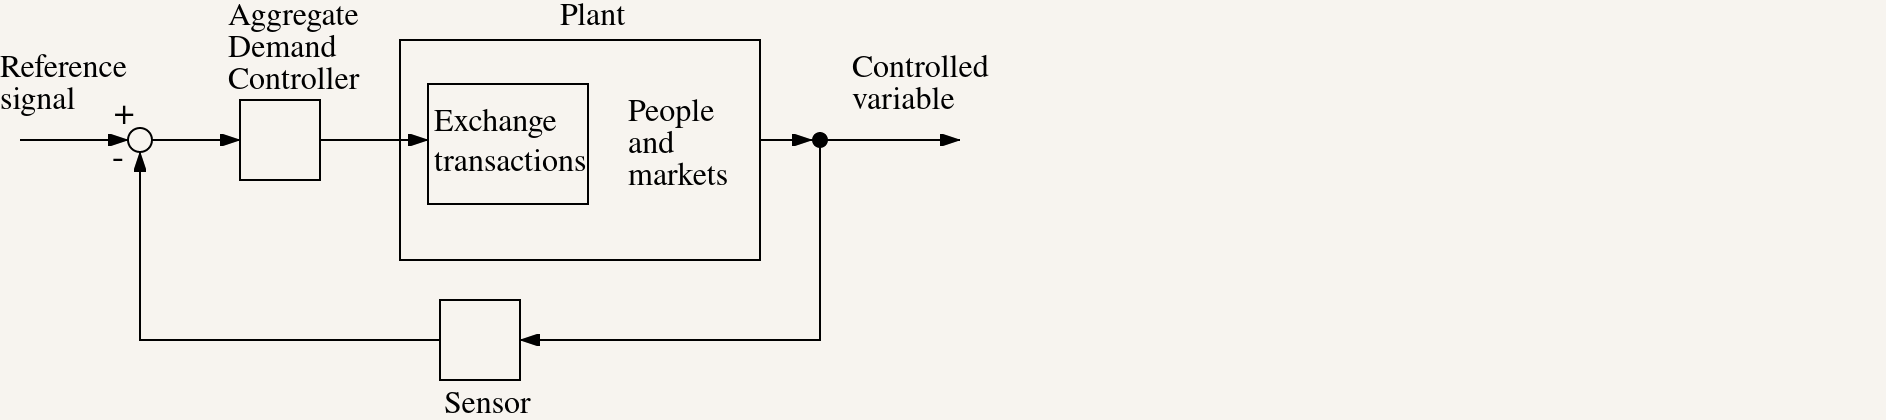
\includegraphics[scale=0.60]{03_exchange_transactions/png/exchange_only_feedback_schema}
\caption{Exchange Only Feedback Schema}
\label{fig:exchange_only_feedback_schema1}
\end{figure}

This diagram represents the global behavior of the system, which is the result of the aggregate
effects of local behaviour. An obvious example, is that market behaviour at the global level is the
result of a distributed system of many people interacting with each other in the context of markets.
This is represented as the ``Market Activity'' box. Another example is that the ``Exchange Tx.'' box
represents aggregate effects of all exchange transactions. We need a way to aggregate from
individual transactions to sum variables that summarize their global, macro-level properties.

\subsection{Price and Quantity}

Starting with exchange transactions

\begin{figure}[H]
\centering
\includegraphics[scale=0.60]{03_exchange_transactions/png/exchange_transaction}
\caption{Exchange Transaction}
\label{fig:exchange_transaction2}
\end{figure}

we want to construct some aggregate variables. These aggregate variables could be sums, averages or
some other kind of measures of centrality. We'll categorize exchange transactions into different
``goods categories''. We'll use this term rather than say ``goods and services'' for brevity and
because it more closely reflects our requirements. We'll assume at this point that these goods
categories are sufficiently well-defined and precise as not to introduce too much noise into our
aggregate measures. For a given currency at a given period of time the transactions, we sum the
quantities for each goods category.

\[
    \left( q_1, \dots, q_N \right)
\]

and then let $pi$ be the average price of these transactions for a given good category. Let $N$ be
the total number of different goods categories. We'll denote the units for these values as

\[
    \left( \left[ q_1 \right], \dots, \left[ q_N \right] \right)
\]

We'll denote the average price for each $q_i$.

\[
    \left( p_1, \dots, p_N \right)
\]

The units for the average prices are 

\[
    \left( \left[ \frac {\$} {p_1} \right], \dots, \left[ \frac {\$} {p_N} \right]  \right)
\]

We cannot sum either these prices or quantities because they can have different units. But each
payment $p_i q_i$ can be summed because its unit, using dimensional analysis, is

\[
    \left[ \frac {\$} {q_i} \right] \left[ q_i \right] = \left[ \$ \right]
\]

So for a given time period, total payments for transactions for a currency is 

\[
    F = p_i q_i + \dots + p_N q_N
\]

We want to construct a aggregate measure of prices. As will become clear later in the paper we want
a measure $P$ that can be used to isolate purchasing power from the inflation rate. For example, if
a person has a certain amount of currency in their account at time $t=0$, and that they can buy a
certain amount with this currency, we want to know how much money they must have in their account at
time $t=1$ so that they can buy the same amount. As written, the notion of ``price level'',
``purchasing power'' and ``amount'' are vague and require mathematical treatment.

Suppose at a given time the transactions with quantites

\[
    \overline Q = \left( q_1, \dots, q_N \right) \textrm{ with corresponding prices } \left( p_1, \dots, p_N \right)
\]

occurs. We'll introduce Alice. We'll feed Alice a 1 dollar and Alice will spend this 1 dollar by
randomly selecting goods categories in such a way that in the limit they purchase quantities all in
proportion to total transactions. In other words,

\[
    \varepsilon_{q_1,\dots,q_n} = c_1 \overline Q
\]

where $c_1$ is a number between $0$ and $1$ and $\varepsilon_{q_1,\dots,q_n}$ is the expected value of
the ``abstract person'''s purchases. The $c_1$ represents the purchasing power of the Alice. It
represents the proportion of all transactions over which Alice has the power to purchase, per
dollar. While purchasing power is the amount of goods that will buy a given unit of currency, the
price level is its reciprocal, the amount of currency that will buy a unit of quantity.

We need to make things more precise, and to check that our measure of price can be used as an index
to isolate Alice's purchasing power from changes in the inflation rate. The motivate for this will
become clear later in the paper.

First we'll do a static analysis, and try to construct meaningful measures of aggregate price and
quantity for a time period that has 

\[
    \overline Q = \left( q_1, \dots, q_N \right) \textrm{ with corresponding prices } \left( p_1, \dots, p_N \right)
\]

Here, the vector $\overline Q$ represents a collection of values, but we want to construct a single
value that is a aggregate of these values. The problem is that each of these values may have
different units. We can construct units that such as ``one apple and two oranges''. The problem is
that if we do this it is impossible to express ``two apples and two oranges'' in these units. But if
we consider only a single period of time that has $\overline Q$ transactions, then we can express
this value in any unit of the form

\begin{equation}\label{equation:basket}
    \left( \left[ \gamma q_1 \right], \dots \left[ \gamma q_N \right] \right)
\end{equation}

for any number $\gamma$. So in fact there is not just one, but a set of feasible units in which to
express $\overline Q$. We refer to any one of these set of units as a ``basket of goods''. Given
that we select one of these sets of units, we can then express $\overline Q$ as some number $Q$,
where the units given by equation (\ref{equation:basket}) with a specific $\gamma$. The units of
$Q$ is this basket of goods. Now we can set the price level as the payment for this basket of goods.
This value $P$ is in units \$ per basket. And so

\[
    F = PQ
\]

The units used depends on the $\overline Q$ at a point in time. Of the proportion of $q_i$ changes
we would have to use a different unit, and so we couldn't do any dynamic analysis (comparisions
across time). We can solve this problem by further constraining our units. As noted, for any
$\overline Q$ at any time we can construct a new unit. We further constrain this by setting the rule
that given one basket of goods whose value of $\gamma$ is arbitrarily chosen, we constrain all other
baskets of goods, by setting their $\gamma$ to a value such that all baskets of goods have the same  
average of quantities weighted by their share of trade.

\begin{equation}
    \gamma' =  \gamma \frac {\varepsilon \left( \left[ q_1 \right], \dots, \left[ q_N \right] \right)}
    {\varepsilon \left( \left[ {q_1}' \right], \dots, \left[ {q_N}' \right] \right)}
\end{equation}

Now, because $\gamma$ depends only the average of the units in the baskets of goods, the distribution of
$q_i$ around this average becomes irrelevant. This means that \textit{however} $\overline Q$
changes, whatever its distribution, the relation $F=PQ$ is exact.  

This section has involved various manipulations of units, most critically the ratio of dollar
payments to a quantity of some good or service of a collection of different quantities of goods and
services. Throughout the paper we will see that questions of units are important. Section
\ref{section:exchange_transactions_and_errors}. will show that the price unit must change over
time. In Section \ref{section:time_transactions}. we show that the price unit written into
contracts must be constant over time. To isolate these different units and construct a control
system that has sufficient degrees of freedom required for control, the use of indices is useful.

\subsection{Aggregate Supply and Demand}
\label{section:aggregate_supply_and_demand}

We can now take a digital currency and measure aggregate properties $F$, $P$ and $Q$ from the set of
transactions. We can also measure their relative change between two time periods.

\[
    \frac {\Delta F} F = \frac {\Delta P} P + \frac {\Delta Q} Q
\]

We'll denote the rate of change of the price level as the inflation rate $I$. We'll denote the rate
of rate of $Q$ as the growth rate $G$, so

\begin{equation}
    \label{equation:fig}
    \frac {\Delta F} F = I + G
\end{equation}]

At the micro-level equilibriation process for a market for a good or service is driven by excess
demand and excess supply. The details of this process are the result of an aggregate of human
decisions and is to a large-extent un-knowable, un-measurable and un-predictable. Nevertheless it is
undeniable that such an equilibriation process exists, and we can abstract this process it a
reaction of prices and quantities to excess supply and excess demand at the level of a market for a
good or service. Excess supply and excess demand can be measures in $\$$, and all the micro-level
values for excess supply and demand can be summed to get a value for aggregate demand $AD$ and
aggregate supply $AS$.  

While we can accurately measure transactions and calculate aggregate properties from these, the
value of $AD$ and $AS$ are less concrete. We can't measure $AD$ directly but we can see its effects
in that if there is no $AD$ or $AS$, then there is nothing to drive prices and quantities which will
therefore remain constant. On the other hand, the unemployment rate is a good measure of excess
$AS$. From $AD$ and $AS$ we can derive a set of agreements, which is the minimum of these two values
(denominated in $\$$), and it is assumed that agreements maps directly to transactions.

\begin{figure}[H]
\centering
\includegraphics[scale=0.48]{03_exchange_transactions/png/agreements}
\caption{Agreements as a function of aggregate supply and demand}
\label{fig:agreements}
\end{figure}

Agreements occur when both sellers and buyers want to transact and so agreements are the minimum of
aggregate supply and aggregate demand as shown in Figure \ref{fig:agreements}.

\subsection{Market Feedback}  
\label{section:market_feedback}

We build here the simplest model that we can think with sufficient explanatory power. The use of
supply and demand models of the decision making processes of economic participants in most useful in
that it encapsulates the notion of markets being driven to equilibrium. We can capture the same
notion by thinking of markets as feedback regulatiors. The value of this model of human behaviour is
not that it is quanititively useful (no-one knows how to predict the decision making process of
economic participants with any accuracy) but that it encapsulates the notion of an equilibriating
process. This process is drive by excess supply and excess demand.

\begin{figure}[H]
\centering

\includegraphics[scale=0.48]{blank}
\caption{Model of a market for a good or service}
\label{fig:micro_feedback}
\end{figure}

The aggregate equilibriation process is driven by the summation of the excess supplys and excess
demands of the individual goods markets it constitutes. We can also model the aggregate
equilibriation process as a feedback regulator.

\begin{figure}[H]
\centering

\includegraphics[scale=0.48]{blank}
\caption{Model of excess aggregate demand/supply response}
\label{fig:macro_feedback}
\end{figure}

In the rest of the paper, only assumption we make about market behaviour is that this simple model
we have presented here is sufficiently accurate for our purposes to explain the behaviour of
markets. Accepting this assumption we focus our attention of the way the design of a currency
impacts on this model.

\subsection{Aggregate Demand Feedback Model}

\begin{figure}[H]
\centering

\includegraphics[scale=0.48]{blank}
\caption{Feedback schema for the control of money supply}
\label{fig:money_supply_feedback}
\end{figure}

\subsection{Market Symmetry}

The model of excess supply and excess demand driving markets to equilibrium is the foundation of
economic theory. The model we have presented is symmetrical in that there is no difference between
markets being driven to equilibrium as a result of excess demand or markets being drive to
equilibrium as a result  

\begin{figure}[H]
\centering
\includegraphics[scale=0.48]{03_exchange_transactions/png/symmetry}
\caption{Symmetric Market Model}
\label{fig:symmetric_market_model}
\end{figure}

In fact if we take unemployment and inflation rate data for all countries we get results like as
shown in Figure \ref{fig:ui_summary}.

\begin{figure}[H]
\centering

\includegraphics[scale=0.48]{blank}
\caption{Unemployment and Inflation Rate}
\label{fig:ui_summary}
\end{figure}

This simple model of supply and demand does not explain macro-economic data very well. The method
invariably used by economists is to try to explain this anomalous behaviour as a property of
decision making by economic participants as they interact in the context of markets. We will take
our cue from David Hume's consideration that currency is important, and so apply methods suitable to
understanding the mechanics of currencies.

\subsection{Control of Price Level}

In Section \ref{section:aggregate_supply_and_demand} we briefly introduced the idea that we could model
macro-level market equilibriation as a feedback regulator, that feeds back excess aggregate supply
and excess aggregate demand back into the price and quantity adjustment process that people engage
in when interacting with others in the context of markets. 

Another important regulation process is the control of the inflation rate through control of
aggregate demand.

Before examining exchange transactions, we will briefly consider the feedback control mechanism.
Indexation is an important method for controlling distributed systems like a currency. An index is a
single value that is utilized by multiple components. An example of indexation in digital currencies
is Bitcoin's method for regulating the rate of production of blocks by Bitcoin miners. In this case
the indexation is algorithmic rather than controlled by a central authority. TODO

Another example of indexation is 

The simplest way to control the price level in a digital currency is to use indexation.





TODO

The feedback control loop does not work, however, in legacy currencies because the core currency
doesn't account for all money. Most money in legacy currencies is banking money, termed M1, M2 and
M3. Under these conditions, money authorities must use alternative methods to try and induce
financial institutions to increase the amount of banking money mainly through changing the interest
rate at which the money authority lends core currency to those financial institutions. At times this
method has been effective at controlling the price level, at other times less so. The process lacks
precision and has a long time-lag, making its use as the main mechanism for controlling economic
conditions problematic. Its effectiveness is also determined by financial institution's ability and
willingness to respond to decreases or increases in the monetary authority's core lending rate in a
way the maps to increases or decreases in aggregate demand.

